\section{Data and Experimental Protocol}
\label{sec:data}

\subsection{Data and outcome}
\label{sec:outcome}

The local training file has 4,500,000 series-day rows and the evaluation file 350,000. A series is a (city, store, product) triple, and the training panel contains 50,000 series. The local training file holds 865 distinct product identifiers, the number given on the current dataset card~\cite{dingdong2025datasetcard}; the pinned dataset report states 863 SKUs~\cite{wang2025freshretailnet}. The card labels the release as version 1.0 under a CC BY 4.0 license. The upstream revision and download date of our copies were not recorded, so the SHA-256 hashes in the availability statement are the only identifiers of the files used.

The outcome is the sum of recorded hourly sales from 06:00 to 21:59, the window a next-day order has to cover, rather than the full-day \texttt{sale\_amount}. A series-day is a donor if its stock-status flags $s_{j,t,h}$ sum to zero over that window; flags outside the window do not matter:
\begin{equation}
\begin{aligned}
I^{\mathrm{donor}}_{j,t}&=\mathbf{1}\!\left\{\sum_{h=6}^{21}s_{j,t,h}=0\right\},\\
\Dproxy_{j,t}&=\sum_{h=6}^{21}y^{\mathrm{sale}}_{j,t,h}
\quad \text{if } I^{\mathrm{donor}}_{j,t}=1.
\end{aligned}
\label{eq:donor}
\end{equation}
On a donor day the recorded window sales equal demand in the window, as long as the flags are correct. The donor set is shaped by the stocking process, however, since low-demand or generously stocked items qualify more often, and results on donors need not hold on censored days. In run~S, fit-period donor days had a pre-day two-week mean of recorded sales 0.91 times that of the other days and fell less often on promotion days (0.35 against 0.39). Real final-week rows with a flagged stockout have no demand label. We never score them for forecast error or order cost; Section~\ref{sec:real} treats them separately.

\subsection{Pipeline and chronological protocol}
\label{sec:protocol}

The pipeline has ten phases: the data contract and sampling (Phase~0), audit and past-only features (1), simulated censoring (2), conventional baselines (3), LightGBM demand quantiles (4), TimesNet and TFT (5), Kaplan--Meier (6), conformal calibration (7), ordering policies and the protocol lock (8), and final evaluation (9). Table~\ref{tab:split} gives the fixed chronological split. Sampling tiers and the initial simulator rules use fit-period data only, hyperparameters are chosen on the tuning window, and the calibration window is used for calibration alone. The 5,000-series samples are stratified by first-level category, sales tier, and stockout-rate tier.

\begin{table}[t]
\centering\footnotesize
\caption{Chronological Split Shared by All Runs}
\label{tab:split}
\begin{tabularx}{\columnwidth}{@{}llc>{\raggedright\arraybackslash}X@{}}
\toprule
Role & Days & Dates & Use \\
\midrule
Model fit & 1--60 & 2024-03-28 to 2024-05-26 & model fitting \\
Tuning & 61--75 & 2024-05-27 to 2024-06-10 & model selection \\
Calibration & 76--90 & 2024-06-11 to 2024-06-25 & calibration only \\
Final & 91--97 & 2024-06-26 to 2024-07-02 & locked evaluation \\
\bottomrule
\end{tabularx}

\end{table}

Features for a target date use only information available before that date. Target-day stockout flags, sales, weather, and promotion values are excluded because they are unknown when the order is placed, and lag and rolling features are shifted by at least one day. The prerequisite audit randomizes every target-day field and confirms that the target-day features do not change. Up to Phase~4, the evaluation file was read for its schema, identifiers, and dates only. Run~E wrote its protocol lock in Phase~8, before any final-week outcome was scored, and the final week has been used once, for the locked evaluation reported here. For each mechanism comparison the target donor keys and dates are identical and only the simulated history differs.

\subsection{Simulated censoring mechanisms}
\label{sec:mechanisms}

Each mechanism replaces the visible history of eligible donor days, those with enough past data, by a simulated censored history; real censored days keep their recorded values. The opening stock of series $j$ on day $t$ under mechanism $m$ is
\begin{equation}
Q^{(m)}_{j,t}=\max\!\left\{\mu^{\mathrm{past}}_{j,t}\,k^{(m)}_{j,t}\exp(\sigma_m z_{j,t}),\;q_{\mathrm{floor}}\right\},
\label{eq:simstock}
\end{equation}
where $\mu^{\mathrm{past}}_{j,t}$ is the mean recorded window sales over the preceding two weeks, $k^{(m)}_{j,t}$ a stock multiplier fitted on fit-period stockout patterns, $z_{j,t}$ a seeded standard normal draw that all mechanisms share, and $q_{\mathrm{floor}}$ a small floor. Visible hourly sales are the lesser of proxy sales and remaining stock. Mechanism~A (ordinary depletion) may add one refill of half the opening stock one to three hours after the first simulated stockout, with a probability estimated from real within-day recoveries. Mechanism~B (promotion-sensitive) follows A but multiplies the stock factor by 0.6 on days that were promotion days in the record, so those days deplete earlier; the promotion flag drives the simulator and is not a forecasting feature. Mechanism~C (sustained scarcity) halves A's multiplier, uses a fixed noise scale, and never refills (Fig.~\ref{fig:mechanisms}). Features are recomputed on every simulated history.

\begin{figure}[t]
\centering
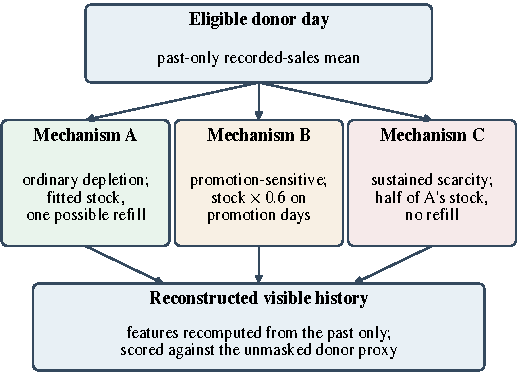
\includegraphics[width=\columnwidth]{figures/mechanism_paths.pdf}
\caption{The three censoring mechanisms act on eligible donor days. Each produces its own visible history, from which past-only features and forecasts are rebuilt; real censored days keep their recorded values.}
\label{fig:mechanisms}
\end{figure}

Within a transfer cell, defined by a training mechanism and an evaluation history, every forecast is scored against the same proxy outcome, so cost differences are paired. Across mechanisms, the masking rate and the distribution of reconstructed features change by design: B probes promotion-linked depletion and C persistent shortage. None of the mechanisms estimates how the retailer would behave under a real change of stocking policy.

\subsection{Models, calibration, and ordering}
\label{sec:models}

The conventional baselines are a seasonal-naive rule and LightGBM~\cite{ke2017lightgbm} point and quantile models trained on visible sales. The demand-quantile family trains LightGBM quantile models on donor-proxy targets at
\[
\tau\in\{0.25,0.50,0.75,0.90\},
\]
with one set per mechanism. On a declared deep subset of series, TimesNet recovers artificially hidden hours and TFT forecasts the next day either from the visible history (direct) or from the TimesNet-recovered history. The Kaplan--Meier policy estimates an order percentile from censored sales within pools that fall back from category by sales tier to category, management group, and a global pool when support is too small. Pooled conformal calibration shifts each quantile by a residual quantile computed on calibration-window donors in the same pool hierarchy, with a minimum pool size of 200, and then sorts the corrected quantiles of each row. The adaptive variant updates its target miss rate after each donor day, as in adaptive conformal inference~\cite{gibbs2021adaptive}, and serves as a sensitivity analysis. Point forecasters (seasonal naive, raw-sales LightGBM, and TFT) become quantile forecasts by adding the pooled quantile of their calibration residuals.

With a cost $c_u$ per unit short and $c_o$ per unit left over, the newsvendor order is the $\beta=c_u/(c_u+c_o)$ quantile of the forecast distribution. The cost of a row is
\begin{equation}
\begin{aligned}
C(Q,\Dproxy)={}&c_o\max(Q-\Dproxy,0)\\
&+c_u\max(\Dproxy-Q,0),
\end{aligned}
\label{eq:cost}
\end{equation}
evaluated against the unmasked donor proxy under a one-day shelf life. The locked settings are $(c_u,c_o,\beta)=(1,3,0.25)$, $(1,1,0.50)$, and $(3,1,0.75)$, which we call excess stock more costly, equal costs, and shortage more costly. Costs are in normalized sales units.

\subsection{Metrics}
\label{sec:metrics}

For a scoring population $\mathcal I$ of donor rows, we report the weighted absolute percentage error of the q50 forecast, the empirical coverage of $q_\tau$, and the pinball loss~\cite{koenker1978regression}:
\begin{align}
\mathrm{WAPE}&=\frac{\sum_{i\in\mathcal I}|\Dproxy_i-\widehat D_i|}{\sum_{i\in\mathcal I}\Dproxy_i}, \\
\widehat C_\tau&=\frac{1}{|\mathcal I|}\sum_{i\in\mathcal I}\mathbf{1}\{\Dproxy_i\le q_{\tau,i}\}, \\
\widehat P_\tau&=\frac{1}{|\mathcal I|}\sum_{i\in\mathcal I}
(\Dproxy_i-q_{\tau,i})(\tau-\mathbf{1}\{\Dproxy_i<q_{\tau,i}\}).
\label{eq:forecastmetrics}
\end{align}
The development files store WAPE as a ratio; the final forecast file stores it as a percentage. Coverage on calibration rows is only a diagnostic, because the same rows set the correction. On donor rows, forecast error, coverage, pinball loss, and order cost answer different questions, and we do not rank methods across them.

For a real final-week row, let $\Sr$ be the recorded window sales and $U_{90}$ the q90 forecast. Demand on a censored row is at least $\Sr$, so every row with $\Sr>U_{90}$ is a certain miss, whereas a row with $\Sr\le U_{90}$ may still hide one. The definite-miss rate
\begin{equation}
L_{\mathrm{miss}}=\frac{1}{n}\sum_{i=1}^{n}\mathbf{1}\{S_{\mathrm{rec},i}>U_{90,i}\}
\label{eq:miss}
\end{equation}
is therefore a lower bound on the real q90 miss rate. It is neither a coverage estimate nor an estimate of censored demand.
